The overview of our implementation is illustrated in
figure~\ref{fig:romc_overview}; one may interpret
figure~\ref{fig:romc_overview} as a depiction of the main class and
the ellipses are the main routines of the class. Following
\proglang{Python}'s naming principles, the methods starting with an
underscore (green ellipses) represent internal (private) functions,
whereas the rest (blue ellipses) are the public methods that the user
interacts with.

Figure~\ref{fig:romc_overview} splits ROMC into the training, the
inference and the evaluation part. The training part includes all the
steps until the computation of the proposal regions i.e. sampling the
nuisance variables, defining the optimization problems, solving them,
constructing the regions and fitting local surrogate models. The
inference part comprises of evaluating the unnormalized posterior (and
the normalized when is possible), sampling and computing an
expectation. From an algorithmic point of view, the training and the
inference parts are \emph{isolated}. We also provide some utilities
for inspecting the training process, such as plotting the histogram of
the final distances or visualizing the constructed bounding
boxes. Finally, in the evaluation part, we provide two methods for
evaluating the inference; (a) computing the Effective Sample Size
(ESS) of the samples and (b) measuring the divergence between the
approximate posterior the ground-truth, if the latter is
available.\footnote{Normally, the ground-truth posterior is not
  available; However, this functionality is useful in cases where the
  posterior can be computed numerically or with an alternative method
  (i.e.\ ABC Rejection Sampling), and we would like to measure the
  discrepancy between the two approximations.}

% \begin{figure}[h]
%     \begin{center}
% 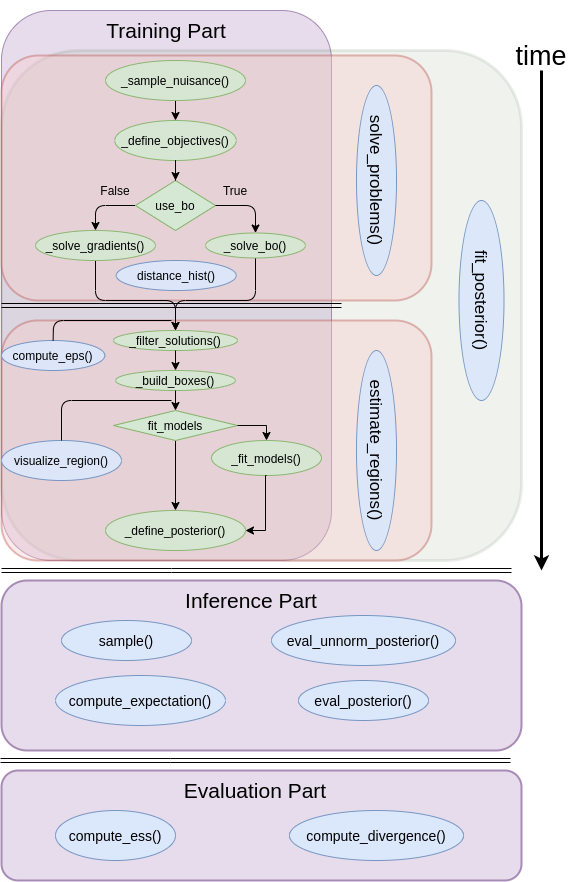
\includegraphics[width=0.5\textwidth]{./latex_files/graphs/ROMC.png}
%     \end{center}
%     \caption[Overview of the ROMC implementation.]{Overview of the
%       ROMC implementation. The training part follows a sequential
%       pattern; the functions in the green ellipses must be called in a
%       sequential fashion for completing the training part and define
%       the posterior distribution. The functions in blue ellipses are
%       the functionalities provided to the user.}
%     \label{fig:romc_overview}
% \end{figure}

\subsubsection*{Parallelizing ROMC method}

ROMC has the significant advantage of being fully parallelizable. We
exploit this fact by implementing a parallel version of all the major
components of the method; (a) solving the optimization problems, (b)
constructing bounding box regions, (c) sampling and (d) evaluating the
posterior. We parallelize these processes using the built-in
\proglang{Python} package \pkg{multiprocessing}. The specific package
enables concurrency, using subprocesses instead of threads, for
side-stepping the Global Interpreter (GIL). For activating the
parallel version of the algorithm, the user simpy has to pass the
argument \code{parallelize=True} when instantiating \code{ROMC}.

\begin{Code}
---------------------------------- python ----------------------------------
>>> elfi.ROMC(<output_node>, parallelize=True)
----------------------------------------------------------------------------
\end{Code}
  
\subsubsection*{Simple one-dimensional example}

For illustrating the functionalities we will use the following running
example introduced by~\cite{Ikonomov2019},

\begin{gather} \label{eq:1D_example}
  p(\theta) = \mathcal{U}(\theta;-2.5,2.5)\\ \label{eq:1D_example_eq_2}
  p(y|\theta) = \left\{
    \begin{array}{ll} \theta^4 + u & \mbox{if } \theta \in [-0.5, 0.5]
\\ |\theta| - c + u & \mbox{otherwise}
    \end{array} \right.\\ 
  u \sim \mathcal{N}(0,1)
\end{gather}

\noindent

The prior is a uniform distribution in the range $[-2.5, 2.5]$ and the
likelihood is defined at~\ref{eq:1D_example_eq_2}. There is only one
observation $y_0 = 0$. The inference in this particular example can be
performed quite easily without using a likelihood-free inference
approach. We can exploit this fact for validating the accuracy of our
implementation.

% \begin{figure}[!h]
%     \begin{center}
% 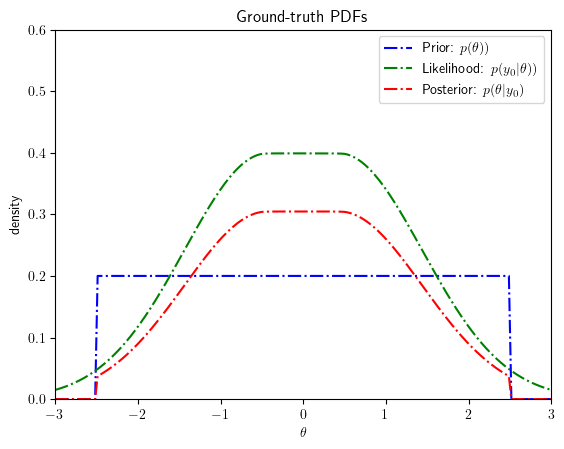
\includegraphics[width=0.7\textwidth]{./latex_files/images/chapter3/example_gt.png}
%     \end{center}
%   \caption[Ground-truth posterior distribution of the simple 1D
% example.]{Ground-truth posterior distribution of the simple 1D
% example.}
%   \label{fig:example_gt}
% \end{figure}

In the following code snippet, we code the model at \pkg{ELFI}.

\begin{Code}
------------------------------ python snippet ------------------------------
  import elfi import scipy.stats as ss
  import numpy as np

  def simulator(t1, batch_size=1,random_state=None):
    if t1 < -0.5:
        y = ss.norm(loc=-t1-c, scale=1).rvs(random_state=random_state)
    elif t1 <= 0.5:
        y = ss.norm(loc=t1**4, scale=1).rvs(random_state=random_state)
    else:
        y = ss.norm(loc=t1-c, scale=1).rvs(random_state=random_state)
    return y

  # observation
  y = 0
      
  # Elfi graph
  t1 = elfi.Prior('uniform', -2.5, 5)
  sim = elfi.Simulator(simulator, t1, observed=y)
  d = elfi.Distance('euclidean', sim)

  # Initialise the ROMC inference method
  bounds = [(-2.5, 2.5)] # limits of the prior
  parallelize = True # activate parallel execution
  romc = elfi.ROMC(d, bounds=bounds, parallelize=parallelize)
----------------------------------------------------------------------------    
\end{Code}
